\textbf{\textcolor{blue}{1.}} Tienes la siguiente sucesión elementos $S = \{5,17,6,8,2,4,1,12,10,3,21\}$. Toma los elementos de dicha sucesión únicamente de izquierda a derecha para los siguientes ejercicios, es decir, el primer elemento a extraer será el $5$, luego el $17$, el $6$, etc... (4 puntos)

\begin{enumerate}

    \item Inserta los 5 primeros elementos dentro de una pila. Saca dos veces el elemento al tope de la pila. Mete los siguientes 4 elementos de $S$. Saca otros 2 elementos de la pila. Por último, ingresa un elemento más. Si sacas todos los elementos de la pila restantes, ¿En qué orden salen? (0.5 pts.)

    \item Inserta los 6 primeros elementos dentro de una cola. Saca 4 elementos de la cola. Ingresa todos los elementos restantes de $S$. Saca otros 3 elementos. Si sacas todos los elementos de la cola restantes, ¿En qué orden salen? (0.5 pts.)
    
    \item Construye un árbol binario ordenado con los elementos de $S$ insertándolos conforme éstos son dados (Ojo, no necesitas balancear el árbol). (0.5 pts.)

    \item Dado el árbol anterior. Realiza una rotación en el nodo que contiene al 17 hacia la derecha. (0.5 pts.)

    \item Ahora sobre el árbol resultante anterior. Realiza una rotación en el nodo que contiene al 6 hacia la izquierda. (0.5 pts.)

    \item Realiza un recorrido BFS sobre el árbol resultante anterior. ¿En qué orden son devueltos los elementos? (0.5 pts.)

    \item Realiza 2 recorridos DFS sobre el árbol resultante del ejercicio 5, uno en pre-orden y otro en post-orden. ¿En qué orden son devueltos los elementos en cada caso? (1 pts.)

\end{enumerate}

$\rhd$\textbf{Solución.}
    \begin{enumerate}
    \item Insertar los 5 primeros elementos dentro de una pila
       \begin{center}
          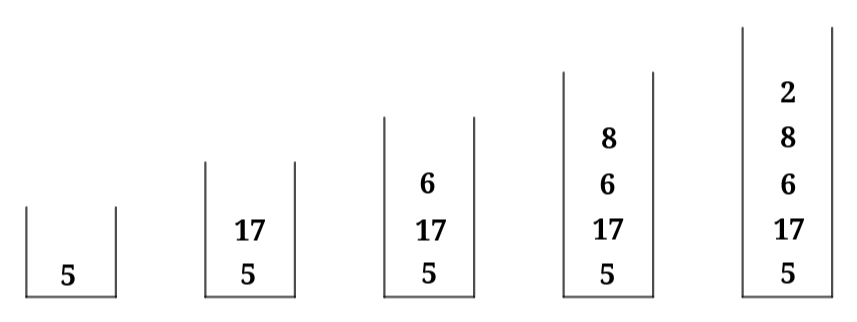
\includegraphics[scale=0.3]{../Image/P1.png}
       \end{center}
       Sacar dos veces el elemento al tope de la pila
       \begin{center}
          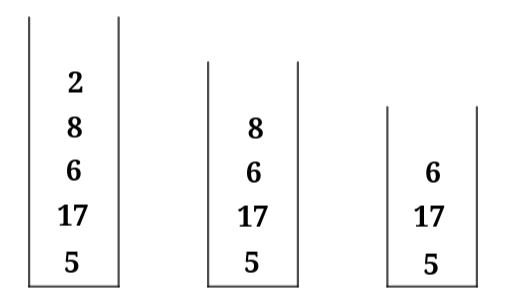
\includegraphics[scale=0.3]{../Image/P2.png}
       \end{center}
       Meter los siguientes 4 elementos de $S$
       \begin{center}
          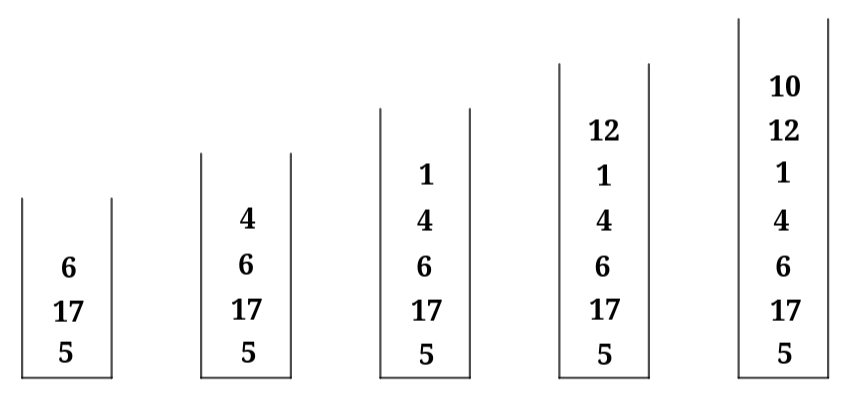
\includegraphics[scale=0.3]{../Image/P3.png}
       \end{center}
       Sacar otros 2 elementos de la pila
       \begin{center}
          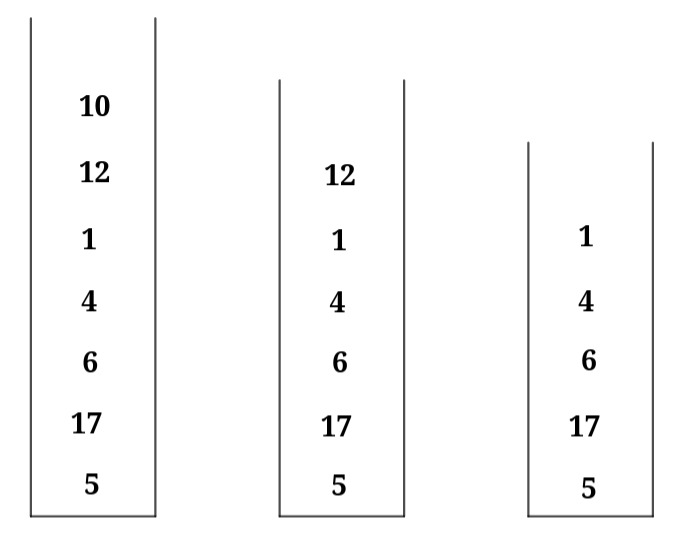
\includegraphics[scale=0.3]{../Image/P4.png}
       \end{center}
       ingresa un elemento más
       \begin{center}
          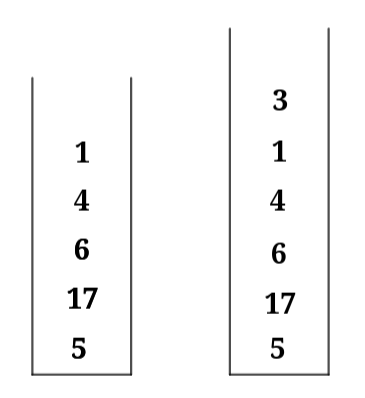
\includegraphics[scale=0.3]{../Image/P5.png}
       \end{center}
       ¿En qué orden salen? [3, 1, 4, 6, 17, 5].
       
       \item Insertar los 6 primeros elementos dentro de una cola
       \begin{center}
          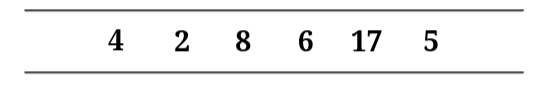
\includegraphics[scale=0.3]{../Image/C1.png}
       \end{center}
       Sacar 4 elementos de la cola
       \begin{center}
          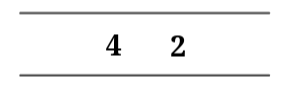
\includegraphics[scale=0.3]{../Image/C2.png}
       \end{center}
       Ingresar todos los elementos restantes de $S$
       \begin{center}
          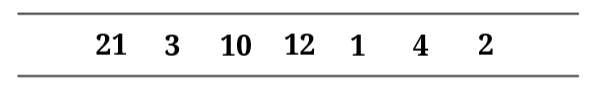
\includegraphics[scale=0.3]{../Image/C3.png}
       \end{center}
       Sacar otros 3 elementos
       \begin{center}
          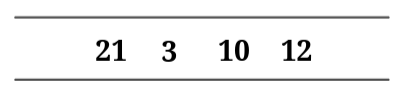
\includegraphics[scale=0.3]{../Image/C4.png}
       \end{center}
       Si sacas todos los elementos de la cola restantes, ¿En qué orden salen? [12, 10, 3, 21].
       \item Construye un árbol binario ordenado con los elementos de $S$ insertándolos conforme
       éstos son dados
       \begin{center}
          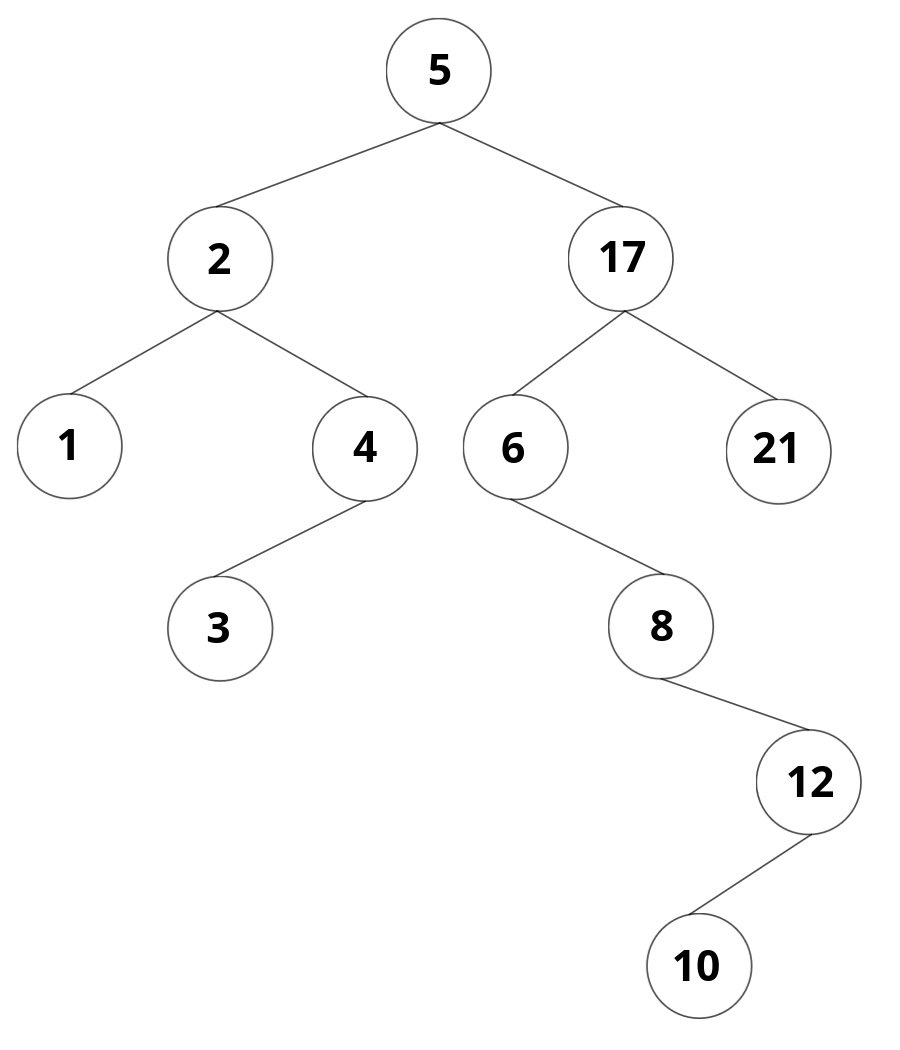
\includegraphics[scale=0.19]{../Image/BST.png}
       \end{center}
       \item Dado el árbol anterior. Realiza una rotación en el nodo que contiene al 17 hacia la derecha
       \begin{center}
          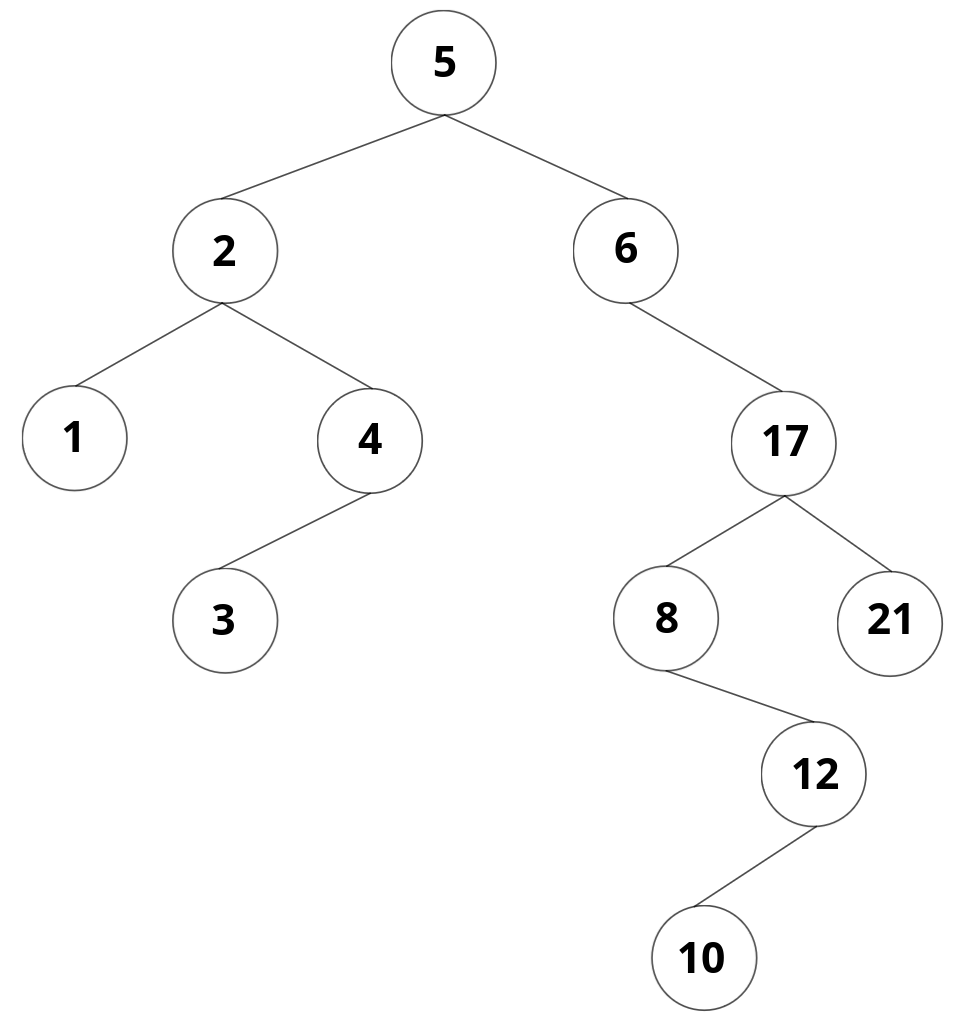
\includegraphics[scale=0.19]{../Image/RD.png}
       \end{center}
       \item Ahora sobre el árbol resultante anterior. Realiza una rotación en el nodo que contiene
       al 6 hacia la izquierda
       \begin{center}
          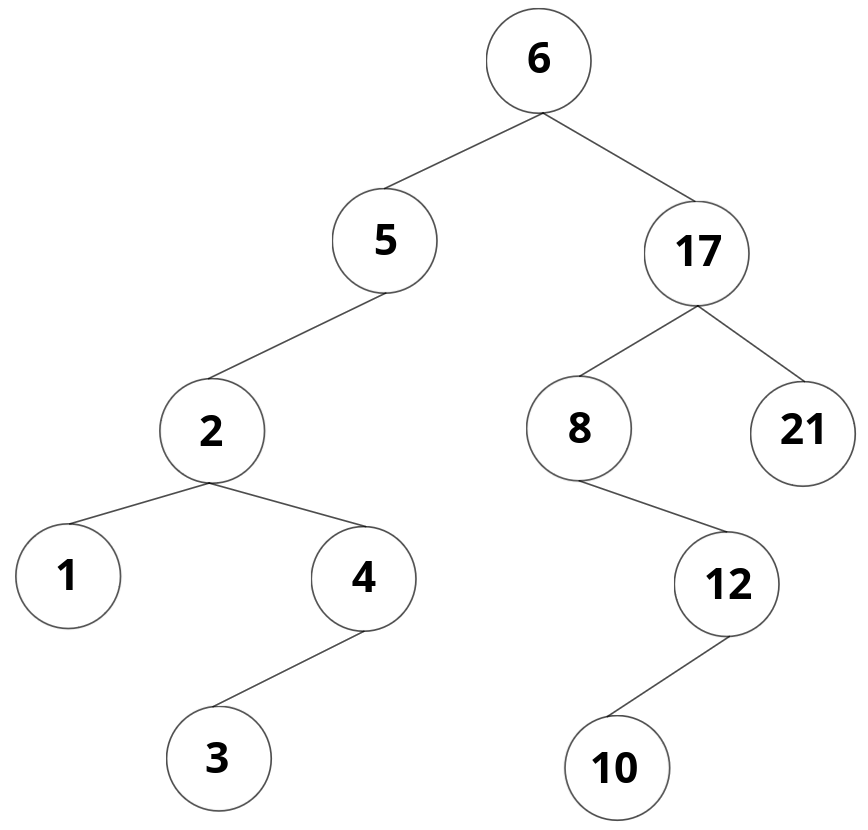
\includegraphics[scale=0.19]{../Image/RI.png}
       \end{center}
       \item Realiza un recorrido BFS sobre el árbol resultante anterior.
       ¿En qué orden son devueltos los elementos? [6, 5, 17, 2, 8, 21, 1, 4, 12, 3, 10].
       \item Realiza 2 recorridos DFS sobre el árbol resultante del ejercicio 5,
       uno en pre-orden y otro en post-orden. ¿En qué orden son devueltos los elementos en cada caso?
       \newcommand{\localtextbulletone}{\textcolor{gray}{\raisebox{.45ex}{\rule{.6ex}{.6ex}}}}
       \renewcommand{\labelitemi}{\localtextbulletone}
       \begin{itemize}
       \item pre-orden: [6, 5, 2, 1, 4, 3, 17, 8, 12, 10, 21].
       \item post-orden: [1, 3, 4, 2, 5, 10, 12, 8, 21, 17, 6].
       \end{itemize}
    \end{enumerate}

\hfill $\lhd$
